\section{Jordfugt} \label{sec:JrdImpl}

Dette afsnit beskriver implementering af SW og HW på PSoC4 i blokken Jordfugt. 

\subsection{HW PSoC4}
\begin{figure}[h]
\centering 
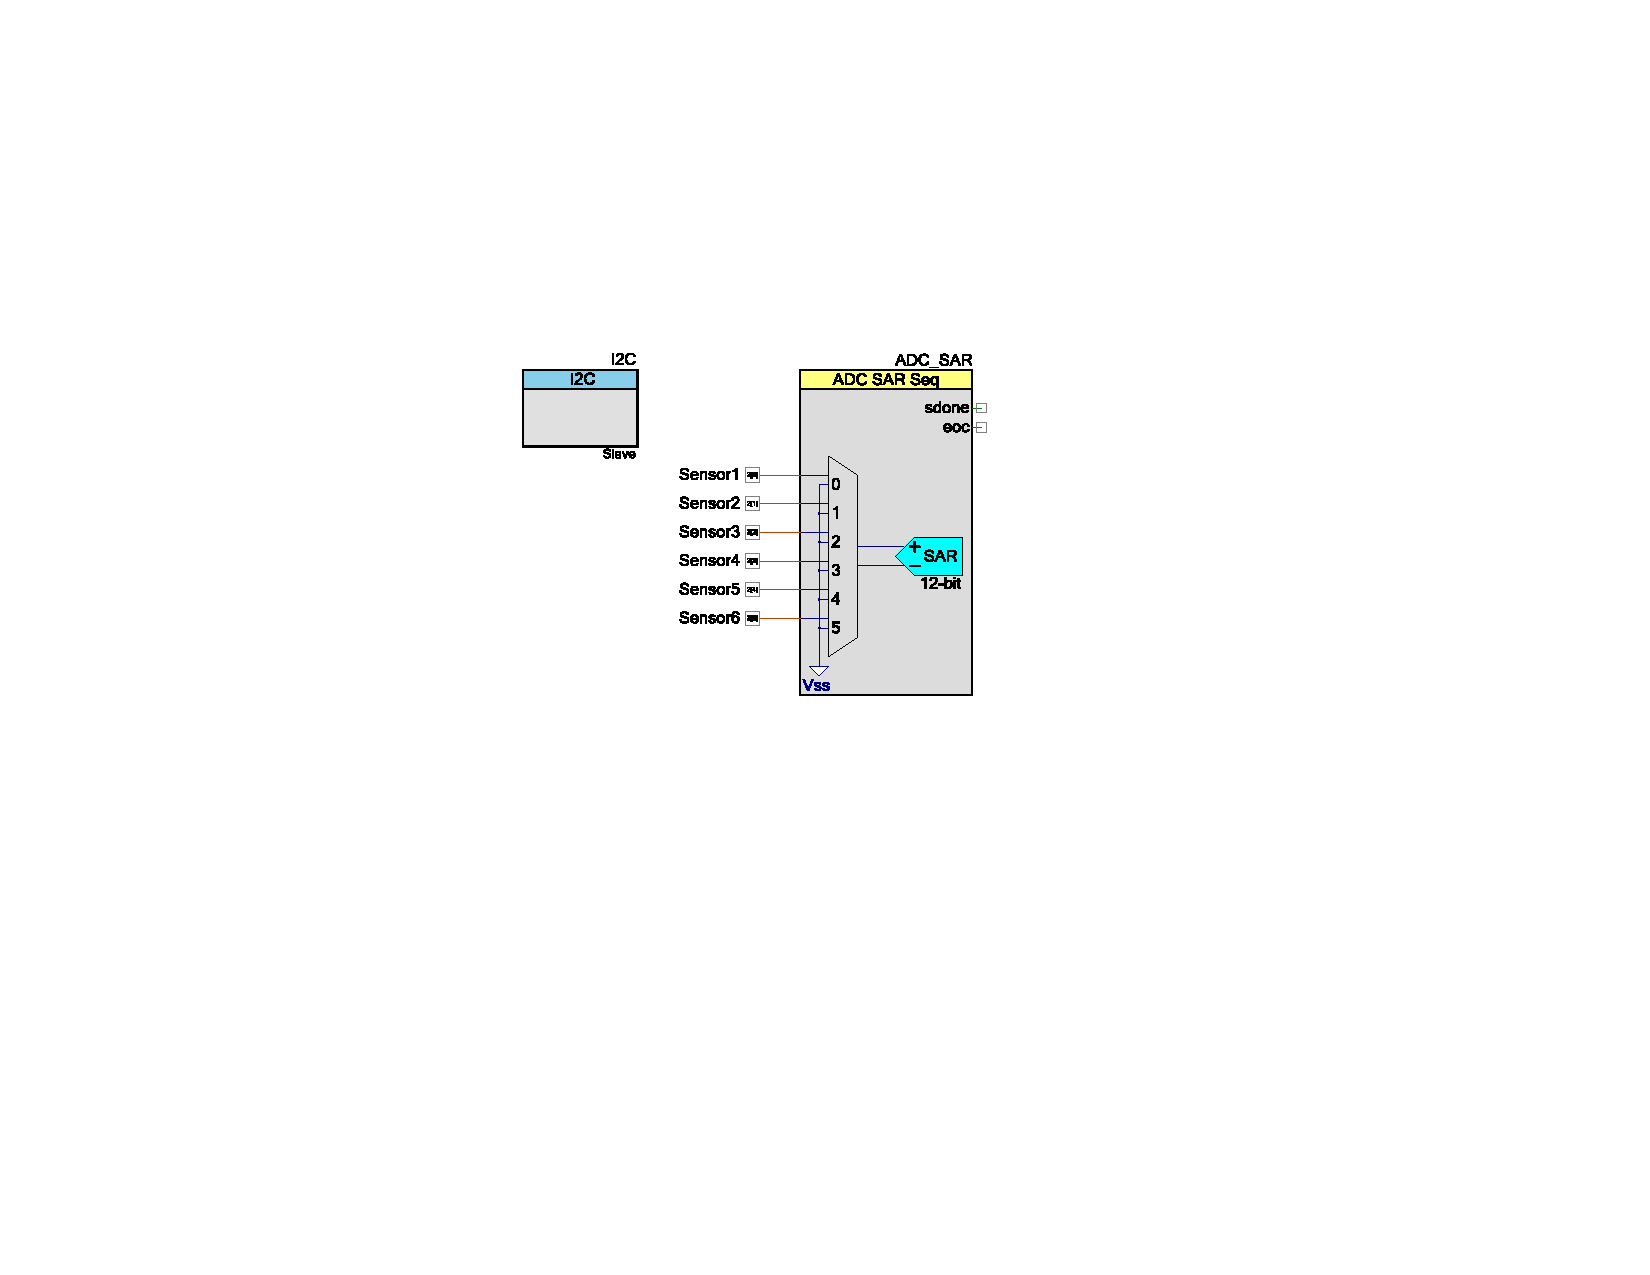
\includegraphics[width={\textwidth-6cm}, trim = 250 270 310 160, clip=true] {../fig/TopDesign_Jordfugt.pdf}
\caption{TopDesign.cysch for PSoC4 i Jordfugt}
\label{fig:topdesign_jordfugt}
\end{figure}

Den HW, der syntetiseres i PSoC4 Jordfugt er vist på Figur \ref{fig:topdesign_jordfugt}. 

Komponenten I2C styrer kommunikation med MasterPSoC via \IIC. 
Den er konfigureret til at være slave med adressen 0x32, datarate er indstillet til 100 kbps.

ADC\_SAR komponenten er en Analog to Digital converter med seks forskellige inputs. Den indeholder seks registre, som opdateres løbende, når den sætets til at køre. Referencespænding er konfigureret til VDDA, dvs. måleområdet er 0V - 3.3V.
Den er desuden indstillet til 8 bit opløsning og en clock frekvens på 1 MHz, hvilket resulterer i en samplerate på 11904 SPS på hver sensor.

Alle pins i topdeignet er konfigureret til high impedans analog, for at undgå spæmdingsdeling med det øvrige kredsløb.

\clearpage

\subsection{SW PSoC4}

\begin{lstlisting}[caption=Udsnit af main.c for PSoC4 i Jordfugt, label=fig:main_jordfugt]
...
	for(;;)
    {
        checkForData();
        if(i < 6)
        {
            data = ADC_SAR_GetResult16(i); //Hent de oenskede data
            //Tjek om oenskede data er inden for graenser
            if ((data & 0b10000000) || (data >= MAXIMUM) || (data < MINIMUM)) 
            {
                convertedData = 0b10000000; //Skriv fejl til konvertede data
            }
            else //Konverter data til tal med vaerdi 1 - 100
            {
                convertedData = (100 - (((data - MINIMUM)*100)/(MAXIMUM-MINIMUM))); 
            }
            readBuffer[0] = convertedData; //Goer data klar til aflaesning
            I2C_I2CSlaveClearReadBuf(); //Reset read buffer pointer
            i = 0xFFFFFFFF;
        }
    }
}
void checkForData()
{
    //Check for om der er modtaget data
    if(I2C_I2CSlaveStatus() & I2C_I2C_SSTAT_WR_CMPLT)
    {
        //Put data i varibel i            
        i = writeBuffer[0] & 0b00000111;
        
        I2C_I2CSlaveClearWriteBuf(); //Clear buffer pointer
        I2C_I2CSlaveClearWriteStatus(); //Clear status                               
    }
}
\end{lstlisting}

Filen main.c, hvoraf den vigtigste del er vist på Listing \ref{fig:main_jordfugt}, fungerer jf. State Machinen på Figur \ref{fig:stm_jordfugt} side \pageref{fig:stm_jordfugt}.

Programmet tjekker om der er modtaget data på \IIC, og opdaterer evt. indexvariablen i til den ønskede jordfugt index. Dette sker vha. funktionen checkForData().

Ud over at opdatere indexvariablen i, cleares pointeren i write bufferen ligeledes i checkForData(), så bufferen er klar til at modtage nye data. 

I tilfælde af at indexvariablen i er blevet opdateret til et sensornummer (0-5), indlæses data fra jordfugtsensoren med det pågældende nummer. Såfremt at dataene ligger inden for grænseværdierne, vil disse data blive konverteret til et tal mellem 1 og 100. Dette tal vil herefter blive skrevet til read bufferen.
I tilfælde af at dataene er uden for grænseværdierne, vil der blive skrevet en fejlværdi til read bufferen.
Grænseværdierne er fastsat ud fra praktiske forsøg, således at helt tør jord giver en lav værdi, og gennemvædet jord giver en værdi tæt på 100. 
Dette er med til at fejlsikre systemet; hvis en sensor ved en fejl er koblet fra, vil SAR'en måle en værdi højere end maximum, og der bliver skrevet en fejlværdi til read bufferen. 
Hvis en sensor er kortsluttet, vil SAR'en måle en værdi under minimum, og det samme vil ske. 

Til slut opdateres indexvariablen i til en værdi, der ikke svarer til et sensornummer.

\clearpage